\newpage
\section{ボリュームを使って\ruby{画像}{が|ぞう}を動かしてみよう}
A0にボリューム(\#104)をつなげてみましょう。HSPスクリプトエディタで\textasciitilde /05/angle.hspを開いて実行してください。\\

\begin{lstlisting}[caption=angle.hsp,label=angle.hsp]
#include "hsp3dish.as"
#include "rpz-gpio.as"

celload("hyou.png"),2
p = 50

spiopen 0

*main
	data = spiget(0,0)
	p = rasp_map(data, 0, 1023, 0, 440)

	redraw 0
	pos 100,100
	mes data
	mes p
	pos 0,0
	celput 2
	redraw 1

	wait 10	
	goto *main

spiclose 0
\end{lstlisting}

画像を使うためには\code{celload}命令を使います。
\code{celload (“画像の名前”),画像の番号}
で画像を読み\ruby{込}{こ}むことができます。読み込んだ画像は\code{celput 画像の番号}で\ruby{表示}{ひょう|じ}することができます。画像や文字の位置は\code{pos}命令を使って決めることができます。\code{pos}命令で画像の位置がどう変わるのか、 図\ref{angle.hsp}を見てみましょう。

\begin{figure}[H]
\centering
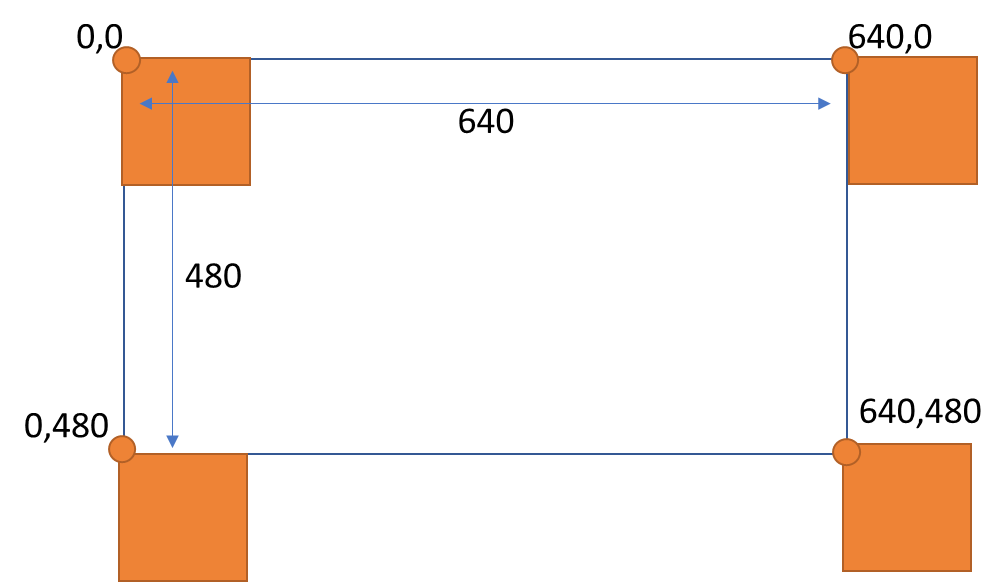
\includegraphics[scale=0.6]{images/chap05/text05-img034.png}
\caption{画面と位置の関係}
\label{angle.hsp}
\end{figure}

\ruby{皆}{みな}さんが使っているHSPでは画面の横のサイズは640、\ruby{縦}{たて}のサイズは480で表示されています。青い四角が画面、オレンジの四角が画像だと思ってください。画像や文字の位置は\code{pos 横の位置,縦の位置}を使って決めます。横の位置は一番左からどれくらい\ruby{離}{はな}れているか、縦の位置は一番上からどれくらい離れているかで決まります。例えば左上は0,0と書くことができます。右下は640,480と書くことができます。一番右上に画像を表示したいとき、640,0と書いてしまうと画像がディスプレイからはみ出てしまいます。\code{pos}命令では画像の左上の点をどこに置くか指定しているからです。画像をディスプレイの中に入れたいときは、画像のサイズ分だけ\code{pos}で指定する位置を左にずらさないといけません。\\

\begin{tcolorbox}[title=\useOmetoi]
\begin{enumerate}
\addex{ボリューム(\#104)をA0につなげて\textasciitilde /05/block3\_angle.hspを実行してみましょう。ボリューム(\#104)を使ってブロック\ruby{崩}{くず}しを遊ぶことができます。}
\addex{angle.hspの pos 0,0 の数字を変えて、右上に画像を表示しましょう。(だいたいで良いです)}
\addex{angle.hspの pos 0,0 の数字を変えて、真ん中に画像を表示しましょう。(だいたいで良いです)}
\addex{angle.hspの pos 0,0 の数字を変えて、左下に画像を表示しましょう。(だいたいで良いです)}
\addex{angle.hspの pos 0,0 の数字を変えて、右下に画像を表示しましょう。(だいたいで良いです)}
\addex{ボリュームを使って画像を横に動かしてみましょう。angle.hspの\code{pos 0,0}を\code{pos p,0}に変えて実行してください。}
\end{enumerate}
\end{tcolorbox}
\begin{tcolorbox}[title=\useOmetoi]
\begin{enumerate}
\addex{時間があったら\ruby{挑戦}{ちょう|せん}してみましょう。前の問題では、ボリュームの\ruby{値}{あたい}を大きくすると、ヒョウが右に動きます。ボリュームの値を大きくしていくと、画像が右から左に動くようにプログラムを変えましょう。\\
ボリュームの入力はdata = spiget(0,0)で受け取り、p = rasp\_map(data, 0, 1023, 0, 440)で値を0~440に\ruby{変換}{へん|かん}します。ボリュームの値で画像を右に動かすには、変数を使います。pには0~440の値が入るため、pos命令で横をpにすればボリュームの値で右に動かすことができます。}
\addex{時間があったら挑戦してみましょう。ボリュームの値で画像が縦に動くようにプログラムを変えましょう。}
\end{enumerate}
\end{tcolorbox}